\documentclass{article}
\usepackage{geometry}
\geometry{
  a4paper,
  margin=0.5in
}

\renewcommand\labelitemi{*}

% Packages
% ------------------
\usepackage{tkz-euclide}
\usepackage{tikz} % for drawing diagrams
\usepackage{bm} % bold mode
\usepackage{subfig}
\usepackage{graphicx}
%% \usepackage{amsfonts}
\usepackage{amssymb}
\usepackage{amsmath}
%% \usepackage{amsthm}
\usepackage{color}
\usepackage{algorithm}
\usepackage{algpseudocode}
\usepackage{dsfont}
\usepackage{forest}

% setup style of tikzlibrary elements
% ------------------------------------
\usetikzlibrary{patterns}
\usetikzlibrary{patterns.meta}
\usetikzlibrary{arrows}
\usetikzlibrary{quotes,angles}
\usetikzlibrary{positioning}
\usetikzlibrary{plotmarks}
\usetikzlibrary{math}
\usetikzlibrary{shapes.geometric, arrows}
\tikzstyle{block} = [rectangle, minimum width=2.5cm, minimum height=1cm, text centered, text width=2.7cm, draw=black, fill=white]
\tikzstyle{redblock} = [rectangle, thick, minimum width=2.5cm, minimum height=1cm, text centered, text width=2.7cm, draw=red, fill=white]
\tikzstyle{wideblock} = [rectangle, minimum width=2.5cm, minimum height=1cm, text centered, text width=5cm, draw=black, fill=white]
\tikzstyle{tallblock} = [rectangle, minimum width=1.9cm, minimum height=2cm, text centered, text width=1.9cm, draw=black, fill=white]
\tikzstyle{inputblock} = [rectangle, minimum width=1.7cm, minimum height=5cm, text centered, text width=1.7cm, draw=black, fill=white]
\tikzstyle{startstop} = [rectangle, rounded corners, minimum width=3cm, minimum height=1cm, text centered, draw=black, fill=white]
\tikzstyle{startstop_wide} = [rectangle, rounded corners, minimum width=6cm, minimum height=1cm, text centered, draw=black, fill=white]
\tikzstyle{io} = [trapezium, trapezium left angle=70, trapezium right angle=110, minimum width=3cm, minimum height=1cm, text centered, draw=black, fill=white]
\tikzstyle{process} = [rectangle, minimum width=4cm, minimum height=1cm, text centered, text width=4cm, draw=black, fill=white]
\tikzstyle{decision} = [diamond, minimum width=3cm, minimum height=1cm, text centered, draw=black, fill=white]
\tikzstyle{arrow} = [->,>=stealth] % can add "thick" to make it bold
\tikzset{radiation/.style={{decorate,decoration={expanding waves,angle=90,segment length=4pt}}}}

%% new commands
% ------------------
\newcommand{\fixme}{\textcolor{red}{\textbf{fix me}} \space}
\newcommand{\attention}[1]{\noindent \fixme \textcolor{red}{#1}}

\definecolor{light-gray}{gray}{0.95}
\newcommand{\code}[1]{\colorbox{light-gray}{\texttt{#1}}}


\begin{document}


% @@@@@@@@@@@@@@@@@@@@@@@@@@@@@@@@@@@@@@@@@@@@@@@@@@

\begin{figure}[h]
\begin{center}
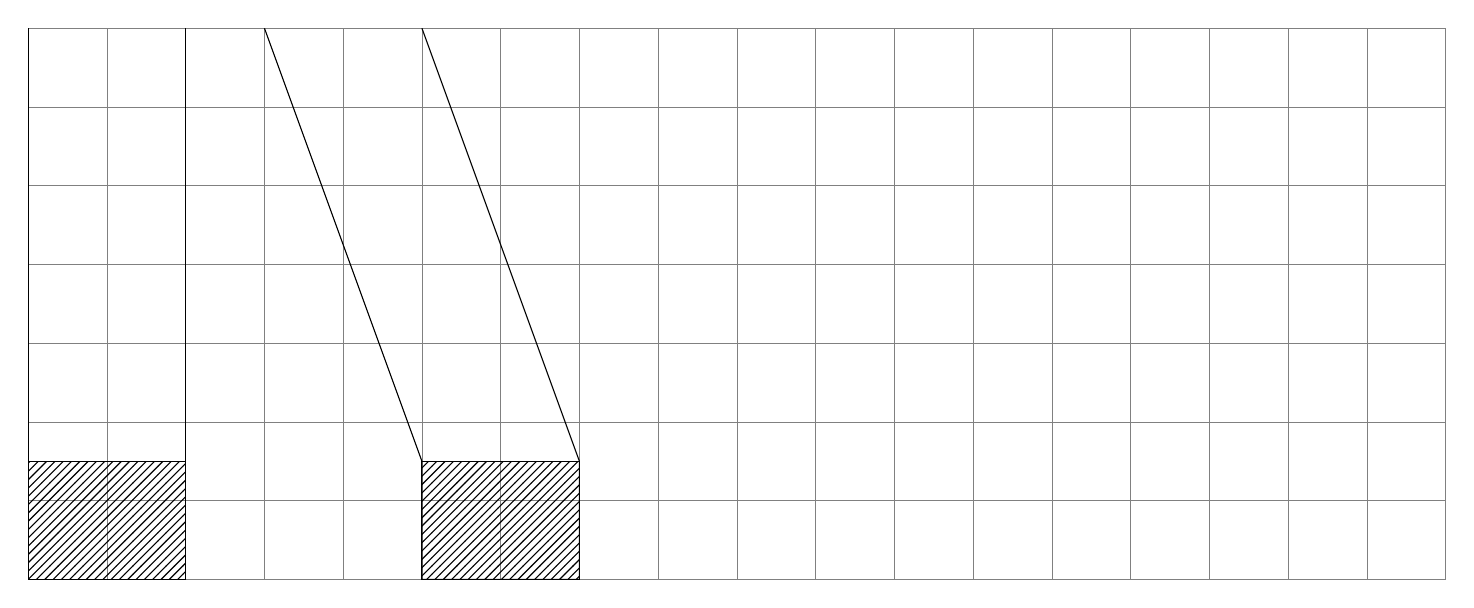
\begin{tikzpicture}[auto, node distance=2.7cm, >=latex']

  \tikzmath{\xmax = 18; \ymax = 7; \width = 2; \bh = 1.5;}
  \tikzmath{\s2 = \width + 1; \s3 = \width*3 + 2;}

  % comment out
  \draw[step=1cm,gray,very thin] (0,0) grid (\xmax,\ymax);

  % Fig 1
  \draw (0,\ymax) -- (0,0) -- (\width,0) -- (\width,\ymax);
  \draw (0,\bh) -- (\width,\bh);
  \draw[pattern={north east lines}] (0,0) rectangle +(\width,\bh);

  % Fig 2
  \draw (\s2,\ymax) -- (\s2+\width,\bh) -- (\s2+\width,0) -- (\s2+\width*2,0) -- (\s2+\width*2,\bh) -- (\s2+\width,\ymax);
  \draw[pattern={north east lines}] (\s2+\width,0) rectangle +(\width,\bh);

  % Fig 3
  \draw (0,\ymax) -- (0,0) -- (\width,0) -- (\width,\ymax);


\end{tikzpicture}
\end{center}
 \caption{Duhem-1905N,fig-1}
\label{fig:Duhem-fig1}
\end{figure}


% @@@@@@@@@@@@@@@@@@@@@@@@@@@@@@@@@@@@@@@@@@@@@@@@@@

% \section{2025.05}
% ---------------------------

\begin{figure}[h]
\begin{center}
\begin{tikzpicture}[auto, node distance=2.7cm, >=latex']

  \tikzmath{\ymax = 16; \b = 1; \tmax = 11;}

  % % comment out
  % \draw[step=1cm,gray,very thin] (0,0) grid (10,\ymax);

  \draw (1,\b) -- (1,\ymax) -- (2,\ymax) -- (2,\b+1);
  \draw (1,\b) arc (180 : 270 : 1cm) node[below left]{C};
  \draw (2,\b+1) arc (180 : 270 : 1cm);

  \draw (2,\b-1) -- (7,\b-1);
  \draw (7,\b-1) arc (270 : 360 : 1cm);

  \draw (3,\b) -- (6,\b);
  \draw (6,\b) arc (270 : 360 : 1cm);

  \draw (7,\b+1) -- (7,\b+2) node[above right]{I};
  \draw (7,\b+2) arc (270 : 180 : 2cm);

  \draw (8,\b) -- (8,\b+2) node[below right]{D};
  \draw (8,\b+2) arc (270 : 360 : 2cm);

  \draw (5,\b+4) -- (5,\tmax) node[left]{E} -- (10,\tmax) node[right]{F} -- (10,\b+4);
  \draw (5,7) -- (5,8) node[left]{C} -- (10,8) node[right]{H} -- (10,7) -- (5,7) node[left]{Q};
  \draw (1,8) node[left]{L} -- (2,8);
  \draw (1,\ymax-3) node[left]{A} -- (2,\ymax-3) node[right]{B};

\end{tikzpicture}
\end{center}
 \caption{Duhem-1905N,fig-4}
\label{fig:Duhem-fig4}
\end{figure}

\newpage


% @@@@@@@@@@@@@@@@@@@@@@@@@@@@@@@@@@@@@@@@@@@@@@@@@@



% -----------------------------
%% \bibliography{references}


% -----------------------------
\end{document}

%%% Local Variables:
%%% mode: latex
%%% TeX-master: t
%%% End:
